\section{Résultats}

\subsection{Extraction du SOS et du EOS}

\`A partir des profils temporels de NDVI obtenus par les 2 méthodes de lissage (HANTS et Whittaker), nous avons extrait le SOS et le EOS respectivement avec les seuils de 10, 20, 30 puis 50\% avant le MAX et 50, 60, 70 puis 80\% après le MAX. Nous avons calculé ensuite pour chacune des parcelles terrain, les écarts en nombre de jours entre les dates de semis et les SOS extraits puis entre les dates de récolte et les EOS estimés. En considérant ces écarts par sytème de culture, nous avons calculé 2 indicateurs statistiques : la racine carrée de l'erreur quadratique moyenne ou \acrshort{rmse} qui est un indicateur d'écart et le coefficient de variation ou \acrshort{cv} qui mesure la dispersion autour la moyenne. 

\paragraph{SOS et évaluation des dates de semis}

La distribution des écarts entre les dates de semis observées et SOS extraits par système de culture et méthode de lissage est illustrée sur la \cref{fig-sosboxplot}. Globalement, les parcelles d'arachide mixte montrent les variabilités les plus faibles entre les écarts calculés (moins de 15 jours maximum d'écart pour tous les seuils) suivies des parcelles de mil pur (moins de 20 jours maximum d'écart pour tous les seuils) et des parcelles de mil mixte qui ont les variabilités les plus fortes (près de 60 jours d'écart avec un seuil de 10\%). Pour l'ensemble des systèmes de culture et presque pour tous les seuils, nous remarquons que la variabilité entre les écarts obtenus avec les SOS Whittaker \footnote{issus des profils lissés par la méthode de Whittaker} est nettement plus faible par rapport à la variabilité entre les écarts obtenus avec les SOS HANTS \footnote{issus des profils lissés par HANTS}. Ceci semble indiquer que la méthode de lissage de Whittaker soit plus appropriée pour estimer le timing du démarrage de croissance de la végétation. Enfin, plus le seuil d'extraction du SOS augmente, plus l'écart entre les dates de semis et le SOS s'accroit, ce qui est tout à fait logique. En ce qui concerne la variabilité de ces écarts, il est assez difficile de dégager le seuil qui les optimise. Pour cela, référons nous à la \cref{fig-sos-rmse-cv} qui montre le RMSE entre SOS et dates de semis en fonction du coefficient de variation de leur écarts pour chaque seuil utilisé et par système de culture. 

\begin{figure}[htbp]
 \begin{center}
  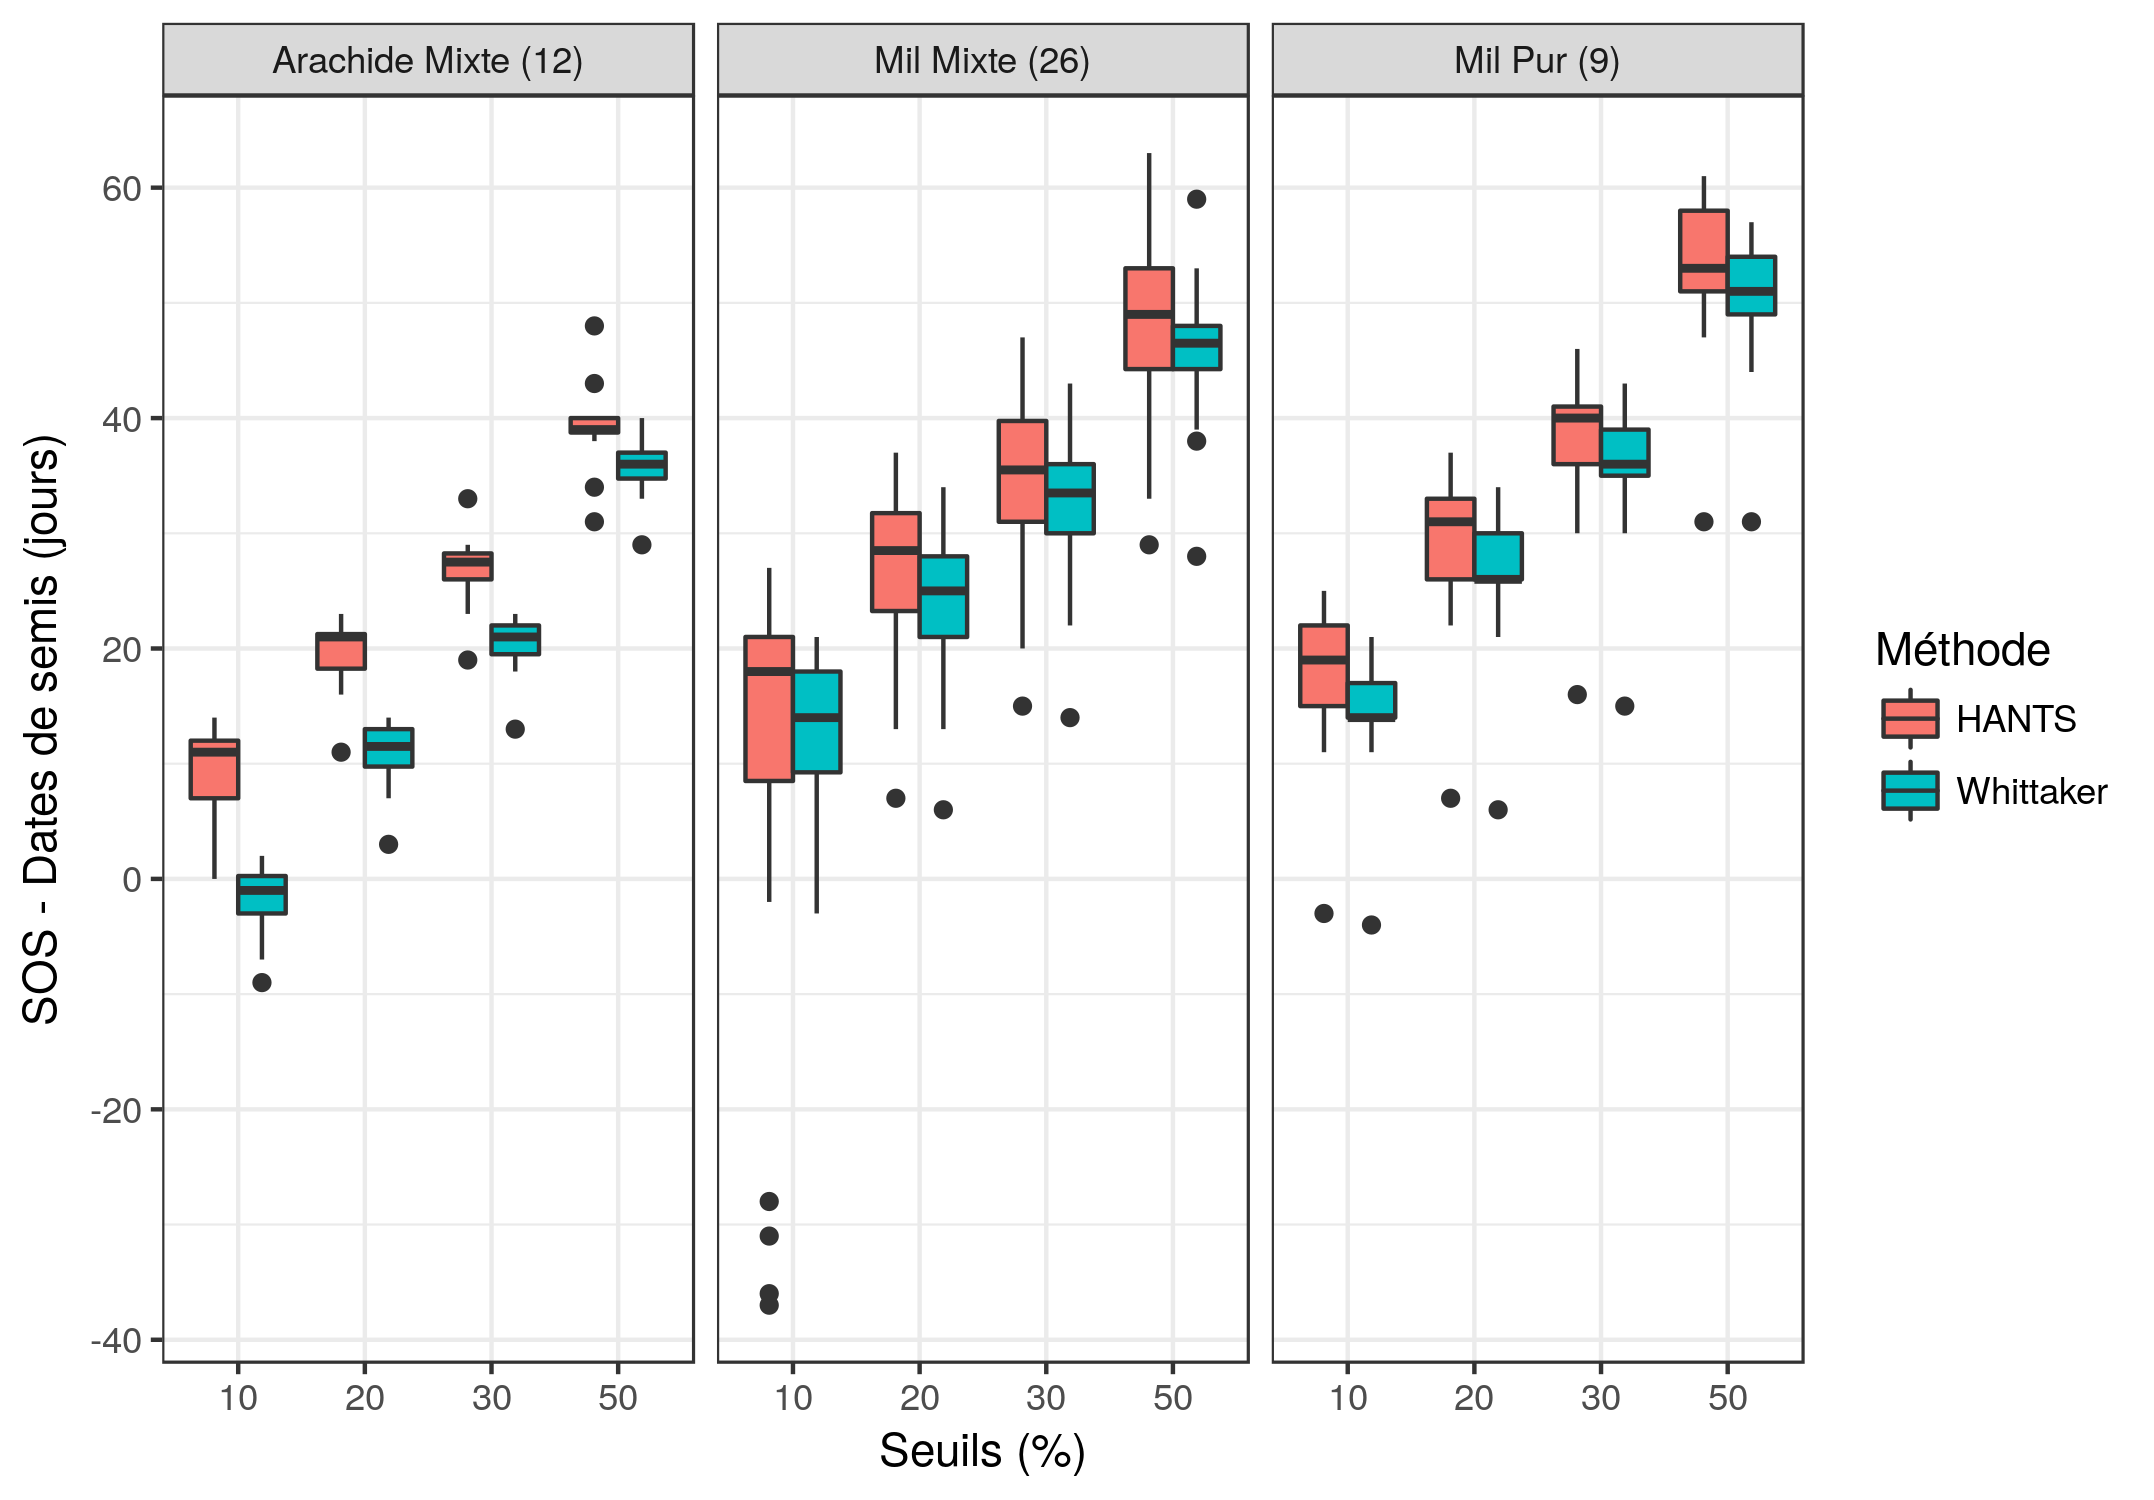
\includegraphics[scale=0.7]{resultats_discussions/SOS_Boxplot.png} 
 \end{center}
 \caption[Distribution des écarts entre SOS et dates de semis]{Boîtes à moustaches illustrant la distribution des écarts entre SOS et dates de semis en fonction des systèmes de culture et des méthodes de lissage}
 \label{fig-sosboxplot}
\end{figure}

\begin{figure}[htbp]
 \begin{center}
  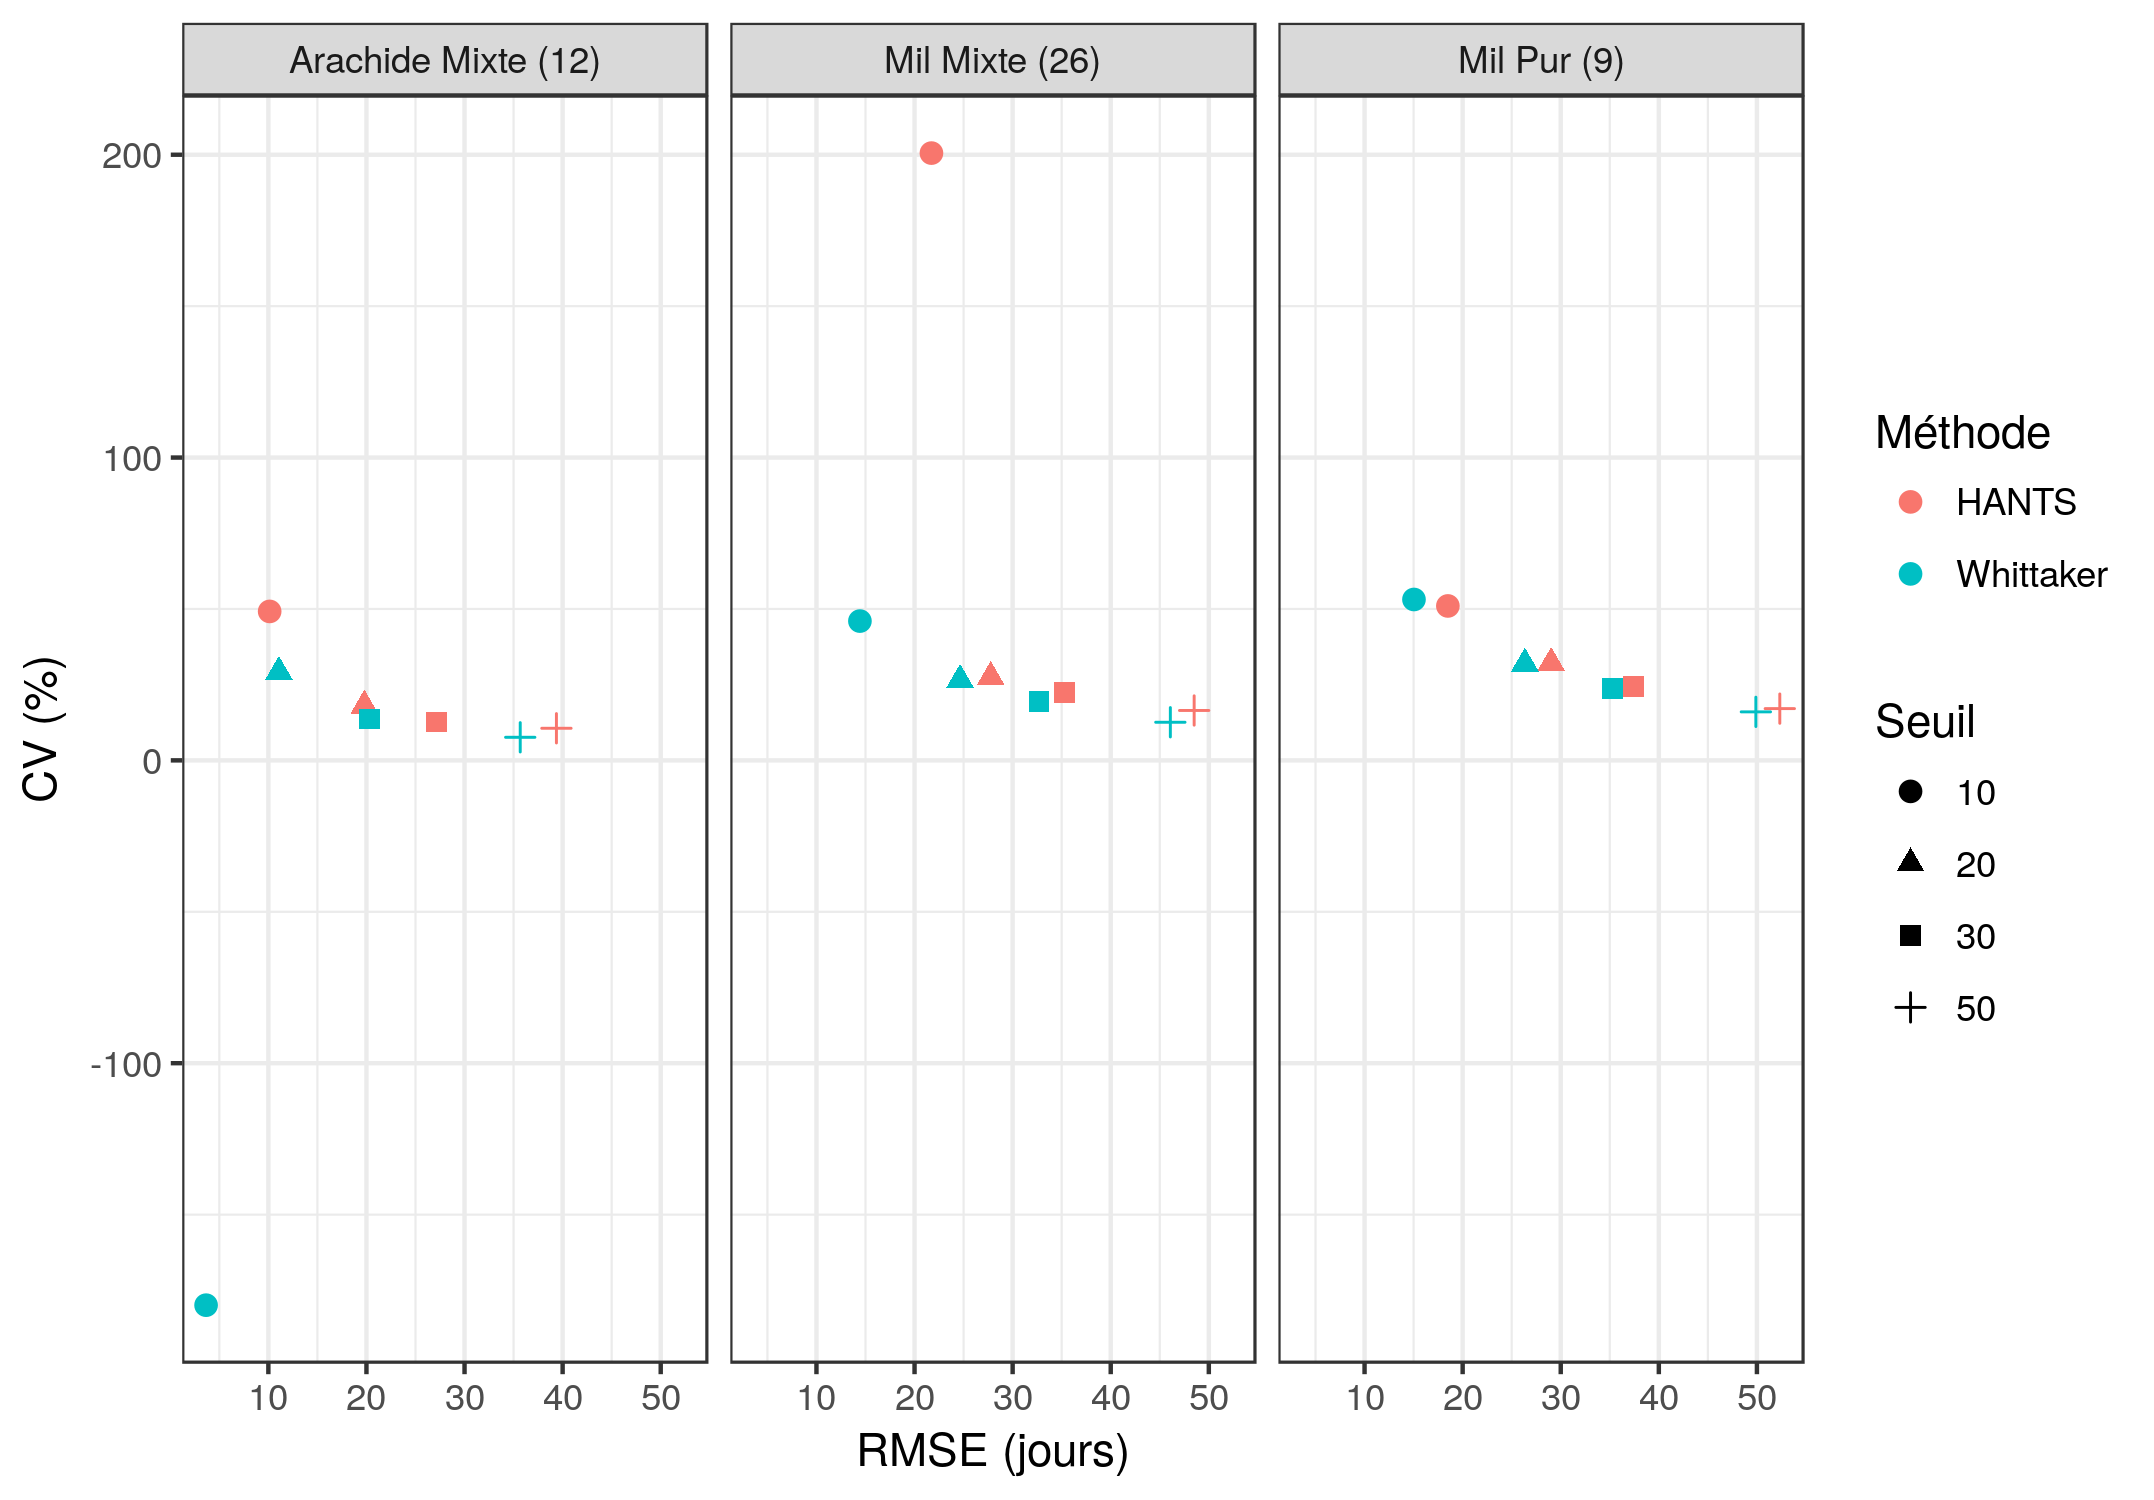
\includegraphics[scale=0.7]{resultats_discussions/SOS_RMSE_vs_CV.png} 
 \end{center}
 \caption{RMSE vs CV}
 \label{fig-sos-rmse-cv}
\end{figure}

\paragraph{EOS}

\subsection{Estimation des rendements}
  
\section{Discussions}

\subsection{Sur l'extraction du SOS et du EOS}

\subsection{Sur l'estimation des rendements}
